\documentclass[12pt]{article}
\usepackage[margin=1in]{geometry}
\usepackage[all]{xy}

\usepackage{amsmath,amsthm,amssymb,color,latexsym}
\usepackage{geometry}        
\geometry{letterpaper}    
\usepackage{graphicx}
\usepackage[utf8]{vietnam}
\newtheorem{problem}{Problem}
\usepackage{listings}
\usepackage{tcolorbox}
\usepackage{verbatim}
\usepackage{tabularx}
\usepackage{array}
\usepackage{colortbl}
\usepackage{xcolor}
\tcbuselibrary{skins}
\definecolor{Salmon}{RGB}{235,235,235}

\newcolumntype{Y}{>{\raggedleft\arraybackslash}X}

\definecolor{codegreen}{rgb}{0,0.6,0}
\definecolor{codegray}{rgb}{0.5,0.5,0.5}
\definecolor{codepurple}{rgb}{0.58,0,0.82}
\definecolor{backcolour}{rgb}{0.95,0.95,0.92}


\definecolor{blockbackgroundcolor}{RGB}{235,235,235}
\definecolor{blockbordercolor}{RGB}{79,79,79}
\newenvironment{solution}[1][\it{Answer}]{\textbf{#1. } }{}
\lstdefinestyle{mystyle}{
    backgroundcolor=\color{backcolour},   
    commentstyle=\color{codegreen},
    keywordstyle=\color{magenta},
    numberstyle=\tiny\color{codegray},
    stringstyle=\color{codepurple},
    basicstyle=\ttfamily\footnotesize,
    breakatwhitespace=false,         
    breaklines=true,                 
    captionpos=b,                    
    keepspaces=true,                 
    numbers=left,                    
    numbersep=5pt,                  
    showspaces=false,                
    showstringspaces=false,
    showtabs=false,                  
    tabsize=2
}

\tcbset{tab1/.style={fonttitle=\bfseries\large,fontupper=\normalsize\sffamily,
colback=yellow!10!white,colframe=red!75!black,colbacktitle=Salmon!40!white,
coltitle=black,center title,freelance,frame code={
\foreach \n in {north east,north west,south east,south west}
{\path [fill=red!75!black] (interior.\n) circle (3mm); };},}}

\tcbset{tab2/.style={enhanced,fonttitle=\bfseries,fontupper=\normalsize\sffamily,
colback=yellow!10!white,colframe=red!50!black,colbacktitle=Salmon!40!white,
coltitle=black,center title}}

\begin{document}
\graphicspath{ {Figs/} } 

\noindent Trí tuệ nhân tạo - CS106.O21 \hfill $A^*$ vs UCS for Sokoban \\
Nguyễn Hoàng Tân - 21521413

\hrulefill


\begin{problem}
	Heuristics được sử dụng có ý nghĩa gì ?
\end{problem}
\hspace{-1em}\textbf{1. Total Manhattan Distance} \\

Đây là một hàm heuristics đơn giản, đầu vào là vị trí các boxes và goals. Đầu tiên chúng ta lọc ra các boxes chưa được đặt vào bất kì goal nào, tương tự lọc các goals chưa đuợc filled bởi box nào. Sau đó, tiến hành bắt cặp và tính khoảng cách \textbf{Manhattan} giữa một box và một goal (Lưu ý, goal được chọn có thể không phải là gần nhất với box đó do tính chất unordered của CTDL set ) \\

\lstset{style=mystyle}

\noindent \hspace*{-1em}\textbf{
	Code Manhattan Heuristics:}
  \begin{tcolorbox}[boxrule=0.5pt, colback=white]
  \begin{lstlisting}[language=python, numbers=none, basicstyle=\ttfamily\footnotesize]
def heuristic_distance(posBox, posGoals):
    """A heuristic function to calculate the overall distance between the else boxes and the else goals"""
    distance = 0
    completes = set(posGoals) & set(posBox)
    sortposBox = list(set(posBox).difference(completes))
    sortposGoals = list(set(posGoals).difference(completes))
    for i in range(len(sortposBox)):
        distance += (abs(sortposBox[i][0] - sortposGoals[i][0])) + 
		            (abs(sortposBox[i][1] - sortposGoals[i][1]))
    return distance
  \end{lstlisting}
  \end{tcolorbox}

  \begin{itemize}
	\item Ưu điểm: Đơn giản, chi phí tính toán thấp + thời gian thực thi nhanh, tìm được lời giải tối ưu trong nhiều trường hợp (14/17 level)
	\item Hạn chế: Chưa xét đến yếu tố PosPlayer (vị trí người chơi), dẫn đến mở các node không cần thiết. Yếu tố địa hình ( PosWall ) cũng chưa được xét đến. Thêm nữa, là việc xảy ra ghép cặp box với goal không phải gần nhất.
  \end{itemize}
\text{\Huge $\Rightarrow$} Ta sẽ thiết kế một heuristics tốt hơn để giải quyết những hạn chế này \\

\hspace{-1em}\textbf{2. Manhattan Distance with PosPlayer and Obtacles} \\

Hãy cùng nhau giải quyết từng vấn đề một
\begin{itemize}
	\item Bắt cặp box với goal gần nhất: \\
	Duyệt qua danh sách boxes và goals chưa được filled, lần lượt tính khoảng cách giữa chúng, chọn ra khoảng cách nhỏ nhất, sau đó loại cặp (box, goal) này ra. Lặp lại quá trình, ta sẽ nhận được các cặp box và goal gần nhất tương ứng.
\begin{tcolorbox}[boxrule=0.5pt, colback=white]
  \begin{lstlisting}[language=python, numbers=none, basicstyle=\ttfamily\footnotesize]
assigned = [0 for _ in range(len(sortposGoals))]

# Only look at boxes that have not been stored
for box in sortposBox:
	closest = float('inf')  
	for goal in sortposGoals:
	# Only look at goals that have not been assigned for a box
	if goal not in assigned:   
	 distance = abs(box[0] - goal[0]) + abs(box[1] - goal[1])
	if distance < closest:
		closest = distance
		assigned[index] = goal
	index += 1
	sum_distance += closest + personalSpace(box, PosOfWalls)
  \end{lstlisting}
  \end{tcolorbox}

  \item Xét đến yếu tố địa hình ( PosOfWalls, Obtacles ): \\
  Khoảng cách Manhattan có thể bị sai lệch do đường đi bị chặn bởi tường hay một box, do đó ta sẽ sử dụng hàm thêm personalSpace được định nghĩa như sau:
  \begin{tcolorbox}[boxrule=0.5pt, colback=white]
	\begin{lstlisting}[language=python, numbers=none, basicstyle=\ttfamily\footnotesize]
def personalSpace(box, obstacles):
	'''Check if any of the 8 neighboring tiles to the box have an obstacle, if they do increase the cost by number of obstacles in this space'''
	personal_space = ((box[0], box[1]+1), (box[0]+1, box[1]), (box[0]-1, box[1]), (box[0], box[1]-1),(box[0]-1, box[1]-1),(box[0]+1, box[1]+1),(box[0]+1, box[1]-1), (box[0]-1, box[1]+1))
	return len(set(personal_space)&set(obstacles)) 
	\end{lstlisting}
	\end{tcolorbox}
	Sau mỗi lần tính khoảng cách gần nhất giữa một box và goal, ta cộng thêm giá trị của personalSpace(box) tương ứng.

	\item Xét đến vị trí của Player (PosOfPlayer): \\
	Trường hợp ta bỏ qua vị trí của Player trong heuristics, thì các hành động không phải đẩy box ( Vị trí các boxes không thay đổi so với state trước ), thì heuricstic sẽ giữ nguyên và nếu cả 4 hướng đều không đẩy box thì 4 hướng đều có cùng một giá trị heuristics. Dẫn đến việc mở các node không cần thiết, thay vào đó các hành động đi hướng đến các cụm boxes nên được ưu tiên hơn. \\

	Ở đây ta sẽ không thêm trực tiếp vào hàm heuristics hiện tại mà sẽ điều chỉnh CTDL PriorityQueue để thêm một \textbf{tie-breaker} value. Khi 2 hoặc nhiều actions có cùng một f-value ( heuristics + cost) thì ta sẽ dùng giá trị này để quyết định node nào nên được mở.

	\begin{tcolorbox}[boxrule=0.5pt, colback=white]
		\begin{lstlisting}[language=python, numbers=none, basicstyle=\ttfamily\footnotesize]
class PriorityQueue:
"""Define a PriorityQueue data structure that will be used"""
def  __init__(self):
	self.Heap = []
	self.Count = 0
	self.len = 0

def push(self, item, priority, tie_breaker = 30):
	entry = (priority, tie_breaker, self.Count, item)
	heapq.heappush(self.Heap, entry)
	self.Count += 1
		\end{lstlisting}
	\end{tcolorbox}

	Giá trị tie-breaker của một node sẽ được tính bằng khoảng cách Manhattan giữa PosPlayer và Centroid của các boxes
	\begin{tcolorbox}[boxrule=0.5pt, colback=white]
		\begin{lstlisting}[language=python, numbers=none, basicstyle=\ttfamily\footnotesize]
def getCenTroidBox(posBox):
	n = len(posBox)
	mean_x = sum(box[0] for box in posBox) / n
	mean_y = sum(box[1] for box in posBox) / n
	return (mean_x, mean_y)
		\end{lstlisting}
	\end{tcolorbox}

	\item Hạn chế việc tính toán lại heuristics không thay đổi: \\
	Như đã nói ở trên, các hành động không phải đẩy boxes thì heuristics sẽ giữ nguyên. Do đó ta sẽ dùng một biến để lưu giá trị heuristics trước đó, nếu PosBox ở state trước và state hiện tại không đổi, ta đơn giản trả về heuristics đã lưu mà không phải tính toán lại.
	
	\item Scale Heuristics: \\
	Do heuristics mới được thiết kế có thêm nhiều yếu tố, nên ta cần scale lại trước khi cộng với cost để tính f-value. Ta sẽ nhân heuristics với trọng số w (Thông qua thực nhiệm, w=0.8 cho kết quả tốt nhất)
	{\large
	\begin{equation}
		f\_value = w*heuristics + cost
	\end{equation}}
	
	\newpage
	\noindent \hspace*{-1em}\textbf{
	Sau khi kết hợp tất cả, ta được đoạn code sau:}
  \begin{tcolorbox}[boxrule=0.5pt, colback=white]
  \begin{lstlisting}[language=python, numbers=none, basicstyle=\ttfamily\footnotesize]
def heuristic_upgrade(posBox, posGoals, PosOfWalls):
    global prev_boxes
    global prev_heuristic
    
    try:
        if prev_boxes == posBox:
            return prev_heuristic
        else:
            prev_boxes = posBox
    except NameError:
        prev_boxes = posBox

    sum_distance = 0
    index = 0
    completes = set(posGoals) & set(posBox)
    sortposBox = list(set(posBox).difference(completes))
    sortposGoals = list(set(posGoals).difference(completes))

    assigned = [0 for _ in range(len(sortposGoals))]

    # Only look at boxes that have not been stored
    for box in sortposBox:
        closest = float('inf') 
        for goal in sortposGoals:
            if goal not in assigned:
                distance = abs(box[0] - goal[0]) + abs(box[1] - goal[1])
                if distance < closest:
                    closest = distance
                    assigned[index] = goal
        index += 1  # Move index incrementation inside the loop
        sum_distance += closest + personalSpace(box, PosOfWalls)
    prev_heuristic = sum_distance  # Update prev_heuristic
    return sum_distance
  \end{lstlisting}
  \end{tcolorbox}
\end{itemize}


\newpage
\begin{problem}
	So sánh UCS và các Heuristics được đề xuất
\end{problem}
	Tiến hành lập bảng thống kê, so sánh các phương pháp trên 3 tiêu chí: Thời gian chạy, Lời giải trả về, Số Node đã mở. \\

\hspace{-1em}\textbf{1. Số Node phải mở} 
\begin{tcolorbox}[tab2,tabularx={X||Y|Y|Y},title=Bảng thống kê số Node đã mở của mỗi thuật toán ứng với từng bản đồ,boxrule=0.5pt]
    \textbf{Level} & \textbf{Heuristics Upgrade} & \textbf{Heuristics} & \textbf{UCS} \\ \hline
    1 & 198 & 208 & 1280 \\ \hline
    2 & 43 & 81 & 131 \\ \hline
    3 & 112 & 99 & 792 \\ \hline
    4 & 47 & 52 & 96 \\ \hline
    5 & 667 & 873 & 562460 \\ \hline
    6 & 515 & 473 & 587 \\ \hline
    7 & 977 & 1224 & 13640 \\ \hline
    8 & 4812 & 5128 & 5254 \\ \hline
    9 & 31 & 61 & 107 \\ \hline
    10 & 430 & 458 & 499 \\ \hline
    11 & 632 & 627 & 649 \\ \hline
    12 & 623 & 1253 & 2806 \\ \hline
    13 & 2131 & 3923 & 5821 \\ \hline
    14 & 4787 & 16748 & 65683 \\ \hline
    15 & 5708 & 5366 & 6283 \\ \hline
    16 & 4712 & 2693 & 108391 \\ \hline
    17 & 169158 & 169158 & 169158 \\ \hline
\end{tcolorbox}

Ta thấy, trong đa số trường hợp, số Node phải mở của thuật toán cải tiến ít hơn hẳn so với thuật toán cũ. Đặc biệt ở level 14, Thuật toán cải tiến mở 4787 nodes trong khi heuristics cũ mở tận hơn 16000 nodes ( \textbf{Chênh lệch 12000 nodes} ).

\begin{figure}[h]
	\hspace{-3em}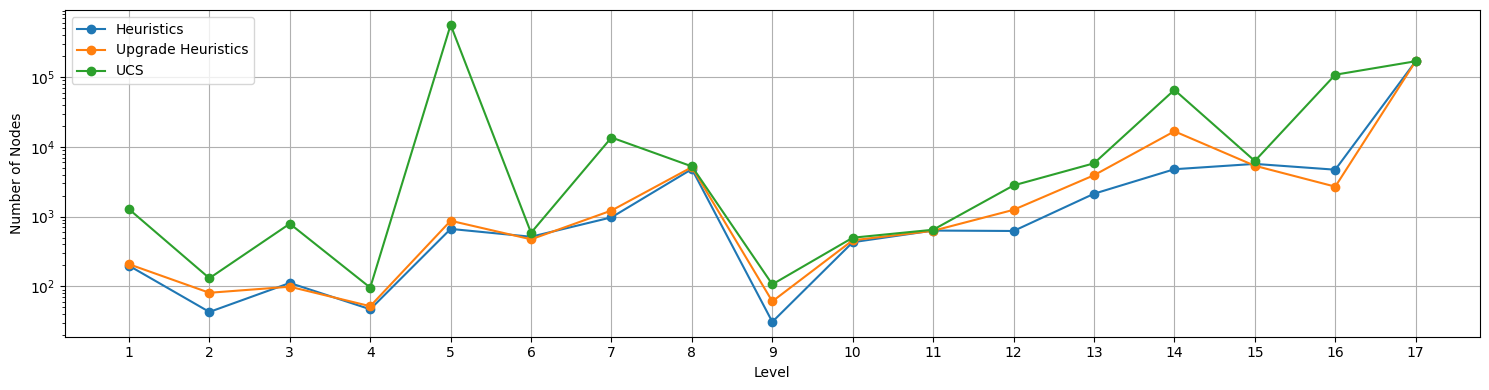
\includegraphics[scale=0.50]{NumberOfNodes.png}
	% \caption{Comparison of Algorithm Performance on Easy Levels (Running Time less than 1s)}
	\begin{flushleft}
		\end{flushleft}
\end{figure}


\label{tab:model_node_performance}
\newpage
\hspace{-1em}\textbf{2. Thời gian chạy} 
\begin{tcolorbox}[tab2,tabularx={X||Y|Y|Y},title=Bảng thống kê thời gian chạy của mỗi thuật toán ứng với từng bản đồ,boxrule=0.5pt]
	\textbf{Level} & \textbf{Heuristics Upgrade} & \textbf{Heuristics} & \textbf{UCS} \\ \hline
	1 & 0.014084 & 0.010208 & 0.052647 \\ \hline
	2 & 0.002616 & 0.00278 & 0.052647 \\ \hline
	3 & 0.011446 & 0.008416 & 0.06424 \\ \hline
	4 & 0.003676 & 0.001706 & 0.00596 \\ \hline
	5 & 0.090826 & 0.091814 & 56.9723 \\ \hline
	6 & 0.023384 & 0.011398 & 0.003707 \\ \hline
	7 & 0.053368 & 0.062573 & 0.422843 \\ \hline
	8 & 0.199957 & 0.216957 & 0.163834 \\ \hline
	9 & 0.004413 & 0.004403 & 0.010275 \\ \hline
	10 & 0.016866 & 0.016081 & 0.014639 \\ \hline
	11 & 0.024557 & 0.014747 & 0.021127 \\ \hline
	12 & 0.027454 & 0.038182 & 0.072329 \\ \hline
	13 & 0.078241 & 0.129165 & 0.141282 \\ \hline
	14 & 0.283939 & 0.886282 & 2.391904 \\ \hline
	15 & 0.267345 & 0.244972 & 0.224162 \\ \hline
	16 & 0.536187 & 0.247331 & 13.132285 \\ \hline
	17 & 23.156627 & 23.686152 & 19.932311 \\ \hline
\end{tcolorbox}

Ta thấy, tuy rằng có quá trình tính toán phức tạp hơn hẳn bản Heuristics cho trước, thời gian hoàn thành của 2 heuristics là không chênh lệch quá nhiều, thậm chí có trường hợp bản Heuristics Upgrade nhanh hơn gấp 3 lần ( Level 14 ), Do số node mở ra được giảm đáng kể và không cần tính lại các heuristics lặp lại.
\label{tab:model_time_performance}

\begin{figure}[h]
	\hspace{-3em}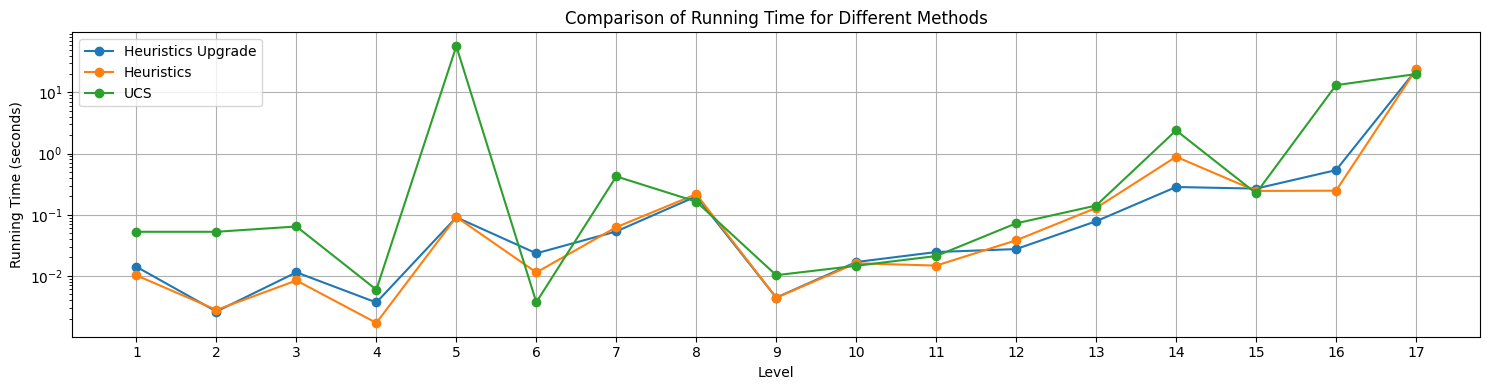
\includegraphics[scale=0.50]{Time.png}
	% \caption{Comparison of Algorithm Performance on Easy Levels (Running Time less than 1s)}
	\begin{flushleft}
		\end{flushleft}
\end{figure}

\newpage
\hspace{-1em}\textbf{3. Lời giải tìm được} 
\begin{tcolorbox}[tab2,tabularx={X||Y|Y|Y},title=Bảng thống kê độ dài lời giải của mỗi thuật toán ứng với từng bản đồ,boxrule=0.5pt]
	\textbf{Level} & \textbf{Heuristics Upgrade} & \textbf{Heuristics} & \textbf{UCS} \\ \hline
	1 & \cellcolor{green!25}12 & 13 & \cellcolor{green!25}12 \\ \hline
	2 & \cellcolor{green!25}9 & \cellcolor{green!25}9 & \cellcolor{green!25}9 \\ \hline
	3 & \cellcolor{green!25}15 & \cellcolor{green!25}15 & \cellcolor{green!25}15 \\ \hline
	4 & \cellcolor{green!25}7 & \cellcolor{green!25}7 & \cellcolor{green!25}7 \\ \hline
	5 & \cellcolor{green!25}20 & 22 & \cellcolor{green!25}20 \\ \hline
	6 & \cellcolor{green!25}19 & \cellcolor{green!25}19 & \cellcolor{green!25}19 \\ \hline
	7 & \cellcolor{green!25}21 & \cellcolor{green!25}21 & \cellcolor{green!25}21 \\ \hline
	8 & \cellcolor{green!25}97 & \cellcolor{green!25}97 & \cellcolor{green!25}97 \\ \hline
	9 & \cellcolor{green!25}8 & \cellcolor{green!25}8 & \cellcolor{green!25}8 \\ \hline
	10 & \cellcolor{green!25}33 & \cellcolor{green!25}33 & \cellcolor{green!25}33 \\ \hline
	11 & \cellcolor{green!25}34 & \cellcolor{green!25}34 & \cellcolor{green!25}34 \\ \hline
	12 & \cellcolor{green!25}23 & \cellcolor{green!25}23 & \cellcolor{green!25}23 \\ \hline
	13 & \cellcolor{green!25}31 & \cellcolor{green!25}31 & \cellcolor{green!25}31 \\ \hline
	14 & \cellcolor{green!25}23 & \cellcolor{green!25}23 & \cellcolor{green!25}23 \\ \hline
	15 & 107 &  \cellcolor{green!25}105 &  \cellcolor{green!25}105 \\ \hline
	16 & 38 & 42 &  \cellcolor{green!25}34 \\ \hline
	17 & \cellcolor{green!25}0 & \cellcolor{green!25}0 & \cellcolor{green!25}0 \\ \hline
	\end{tcolorbox}
\label{tab:model_performance}
\begin{flushleft}
	Note: Ô màu xanh nghĩa là lời giải tối ưu
\end{flushleft}
Ta thấy, Heuristics Upgrade luôn tìm ra thời giải tốt hơn hàm Heuristics cơ bản, tìm được 14/17 lời giải tối ưu cho các levels, trong khi con số này của hàm Heuristics cũ là 13/17. UCS trong trường hợp này, lời giải tìm được toàn bộ là lời giải tối ưu. Trường hợp duy nhất Heuristics cũ thể hiện tốt hơn Heuristics Upgrade là ở level 15 (107 so với 105). Trong tất cả trường hợp còn lại Heuristics Upgrade luôn tốt hơn.

\begin{figure}[h]
	\hspace{-3em}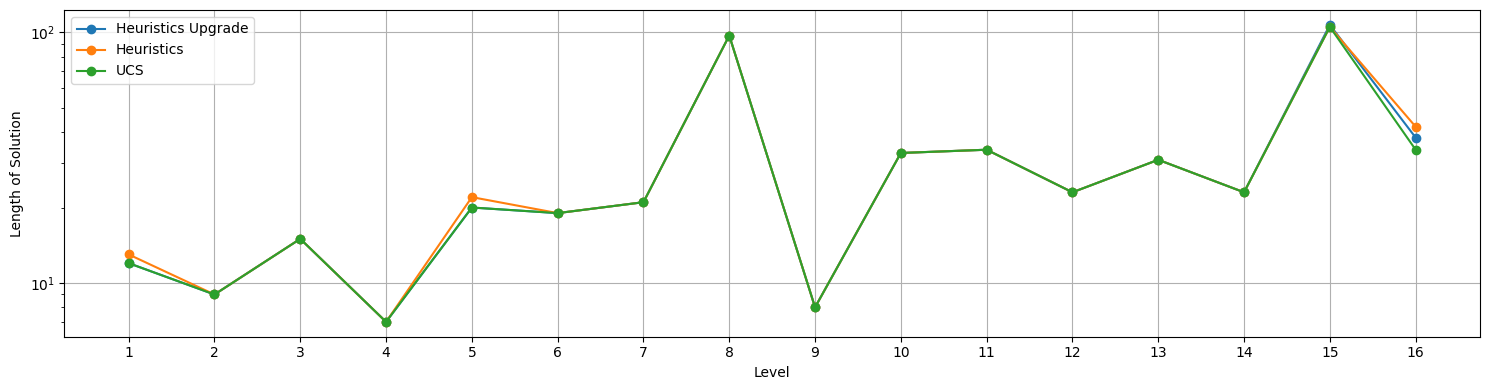
\includegraphics[scale=0.50]{NumberOfMoves.png}
\end{figure}


\end{document}
